%!TEX program = xelatex
%!TEX root = geometria_analitica.tex
%%Usar makeindex -s indexstyle.ist arquivo.idx no terminal para gerar o {\'\i}ndice remissivo agrupado por inicial
%%Ap\'os executar pdflatex arquivo

\chapter{Reta e Plano no Espa\c{c}o} % (fold)
\label{cha:reta_e_plano_no_espaco}

\section{Equa\c{c}\~oes do Plano} % (fold)
\label{sec:equacoes_do_plano}

Da Geometria plana, sabemos que todo plano $\pi$ cont\'em pelo menos tr\^es pontos n\~ao colineares, digamos $A$, $B$ e $C$. Assim considere os vetores
\begin{align*}
    \vec{u} = \vec{AB}\\
    \vec{v} = \vec{AC}.
\end{align*}
Como $\vec{u}$ e $\vec{v}$ n\~ao s\~ao paralelos, ent\~ao podemos considerar o vetor $\vec{u}\times\vec{v}\ne \vec{0}$.
\begin{figure}[!h]
    \centering
    \caption{Equa\c{c}\~ao do plano}\label{definicao-plano}
    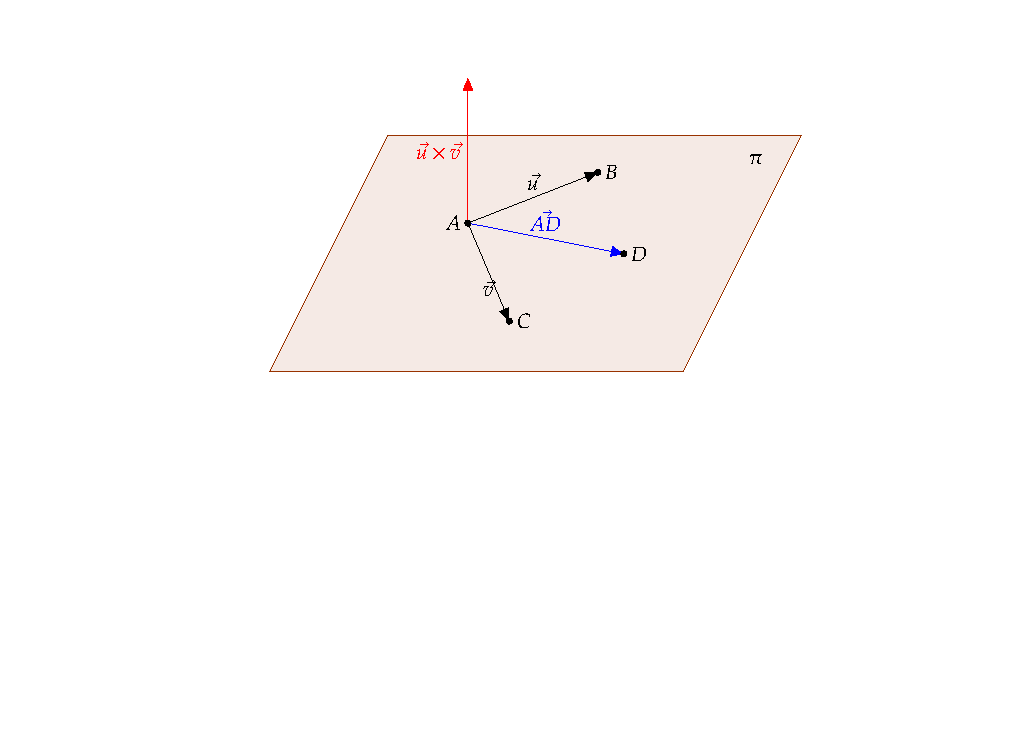
\includegraphics{equacao-plano.pdf}
    % \definecolor{zzttqq}{rgb}{0.6,0.2,0}
    % \definecolor{qqqqff}{rgb}{0,0,1}
    % \begin{tikzpicture}[line cap=round,line join=round,>=triangle 45,x=1.0cm,y=1.0cm]
    %     \clip(-4.3,-6.08) rectangle (12.58,6.3);
    %     \fill[color=zzttqq,fill=zzttqq,fill opacity=0.1] (0,0) -- (2,4) -- (9,4) -- (7,0) -- cycle;
    %     \draw [color=zzttqq] (0,0)-- (2,4);
    %     \draw [color=zzttqq] (2,4)-- (9,4);
    %     \draw [color=zzttqq] (9,4)-- (7,0);
    %     \draw [color=zzttqq] (7,0)-- (0,0);

    %     \coordinate[label=left:$A$] (A) at (3.36,2.52);
    %     \coordinate[label=right:$B$] (B) at (5.56,3.38);
    %     \coordinate[label=right:$C$] (C) at (4.06,0.86);
    %     \coordinate[label=right:$D$] (D) at (6,2);

    %     \coordinate (E) at (3.36,4.98);
    %     \draw [->] (A) -- (B) node[midway,above]{$\vec{u}$};
    %     \draw [->] (A) -- (C) node[midway,below]{$\vec{v}$};
    %     \draw [->,color=blue] (A) -- (D) node[midway,above]{$\vec{AD}$};
    %     \draw [->,color=red] (A) -- (E) node[midway,left]{$\vec{u}\times\vec{v}$};
    %     \foreach \p in {A,B,C,D} \fill (\p) circle (0.5mm);
        
    %     \coordinate[label=right:$\pi$] (P) at (8,3.6);
    % \end{tikzpicture}
\end{figure}
Assim, na Figura \ref{definicao-plano} vemos que um ponto $D$ pertence ao plano $\pi$ se, e somente se, $\vec{u}\times\vec{v} \perp \vec{AD}$. Logo um plano $\pi$ \'e um conjunto de vetores perpendiculares a um dado vetor.

Fixe ent\~ao um ponto $P_0$ em $\real^3$ e $\vec{v}\ne \vec{0}$ um vetor. Passando por $P_0$ existe um \'unico plano $\pi$ perpendicular ao vetor $\vec{v}$. Assim um ponto $P$ do espa\c{c}o pertence ao plano $\pi$ se, e somente se, $\vec{P_0P} \perp \vec{v}$, isto \'e,
\begin{equation}\label{equacaoplanovetorial}
    \vec{P_0P}\cdot\vec{v} = 0.
\end{equation}
Sejam $\vec{v} = (a,b,c)$ um vetor, $P_0(x_0, y_0, z_0)$ e $P(x, y, z)$ pontos em $\real^3$. Logo $\vec{P_0P} = (x - x_0, y - y_0, z - z_0)$ e ent\~ao da equa\c{c}\~ao \eqref{equacaoplanovetorial} obtemos
\begin{equation}\label{equacaoplano}
    (x - x_0)a + (y - y_0)b + (z - z_0)c = 0.
\end{equation}

A equa\c{c}\~ao \eqref{equacaoplano} \'e chamada de \textbf{equa\c{c}\~ao cartesiana do plano} $\pi$. O vetor $\vec{v}$ \'e chamado de \textbf{vetor normal} ao plano $\pi$.\index{Plano!Equa\c{c}\~ao Param\'etrica}\index{Plano!Vetor Normal}

\begin{exemplos}
    Encontre a equa\c{c}\~ao do plano $\pi$ nas seguintes situa\c{c}\~oes:
    \begin{enumerate}
        \item O vetor normal \'e $\vec{v} = (1,2,-1)$ e o ponto de $\pi$ \'e $P_0(1,3,-1)$.
        \begin{solucao}
            Se $P(x,y,z)$ pertence a $\pi$, ent\~ao
            \begin{align*}
                &\vec{P_0P}\cdot\vec{v} = 0\\
                &(x - 1, y - 3, z + 1)\cdot(1,2,-1) = 0\\
                &x - 1 + (y - 3)2 + (z + 1)(-1) = 0.
            \end{align*}
            Logo a equa\c{c}\~ao do plano procurado \'e
            \[
                x + 2y - z - 8 = 0.
            \]
        \end{solucao}
        \item O vetor normal \'e $\vec{v} = (0,0,1)$ e $P_0(0,0,0)$.
        \begin{solucao}
            Se $P(x,y,z)$ pertence a $\pi$, ent\~ao
            \begin{align*}
                \vec{P_0P}\cdot\vec{v} = 0\\
                (x, y, z)\cdot(0,0,1) = 0.
            \end{align*}
            Logo a equa\c{c}\~ao do plano procurado \'e
            \[
                z = 0.
            \]
            \begin{figure}[!h]
                \centering
                \caption{Plano $z = 0$}
                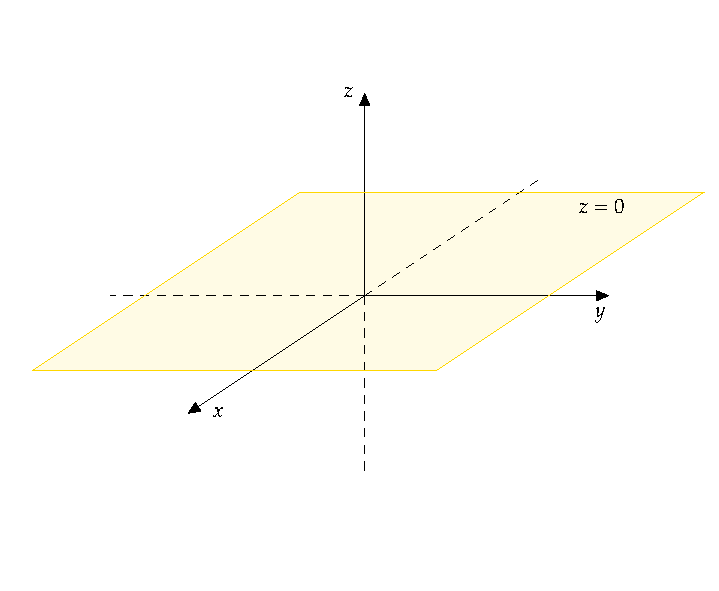
\includegraphics{plano-z=0.pdf}
                % \definecolor{ffdxqq}{rgb}{1.0,0.8431372549019608,0.0}
                % \begin{tikzpicture}[line cap=round,line join=round,>=triangle 45,x=1.0cm,y=1.0cm]
                %     \clip(-6.0,-5.0) rectangle (6.0,5.0);
                %     \fill[color=ffdxqq,fill=ffdxqq,fill opacity=0.1] (-1.0991194968553457,1.751698113207547) -- (5.7463471698113215,1.751698113207547) -- (1.2187999999999999,-1.2666666666666666) -- (-5.626666666666666,-1.2666666666666666) -- cycle;
                %     \draw [->] (0.0,0.0) -- (0.0,3.44);
                %     \draw [->] (0.0,0.0) -- (4.14,0.0);
                %     \draw [->] (0.0,0.0) -- (-3.0,-2.0);
                %     \draw [dash pattern=on 4pt off 4pt] (0.0,0.0)-- (-4.3,0.0);
                %     \draw [dash pattern=on 4pt off 4pt] (0.0,0.0)-- (0.0,-3.0);
                %     \draw [dash pattern=on 4pt off 4pt] (0.0,0.0)-- (3.0,2.0);
                %     \draw [color=ffdxqq] (-1.0991194968553457,1.751698113207547)-- (5.7463471698113215,1.751698113207547);
                %     \draw [color=ffdxqq] (5.7463471698113215,1.751698113207547)-- (1.2187999999999999,-1.2666666666666666);
                %     \draw [color=ffdxqq] (1.2187999999999999,-1.2666666666666666)-- (-5.626666666666666,-1.2666666666666666);
                %     \draw [color=ffdxqq] (-5.626666666666666,-1.2666666666666666)-- (-1.0991194968553457,1.751698113207547);
                %     \draw (-2.696314847942755,-1.7600000000000011) node[anchor=north west] {$x$};
                %     \draw (3.759212880143111,-0.060000000000001136) node[anchor=north west] {$y$};
                %     \draw (-0.4772271914132387,3.659999999999999) node[anchor=north west] {$z$};
                %     \draw (3.512647584973165,1.759999999999999) node[anchor=north west] {$z=0$};
                % \end{tikzpicture}
            \end{figure}
            Agora, se $\vec{v} = (0,1,0)$ e $P_0(0,0,0)$, ent\~ao a equa\c{c}\~ao do plano ser\'a $y = 0$.
            \begin{figure}[!h]
                \centering
                \caption{Plano $y = 0$}
                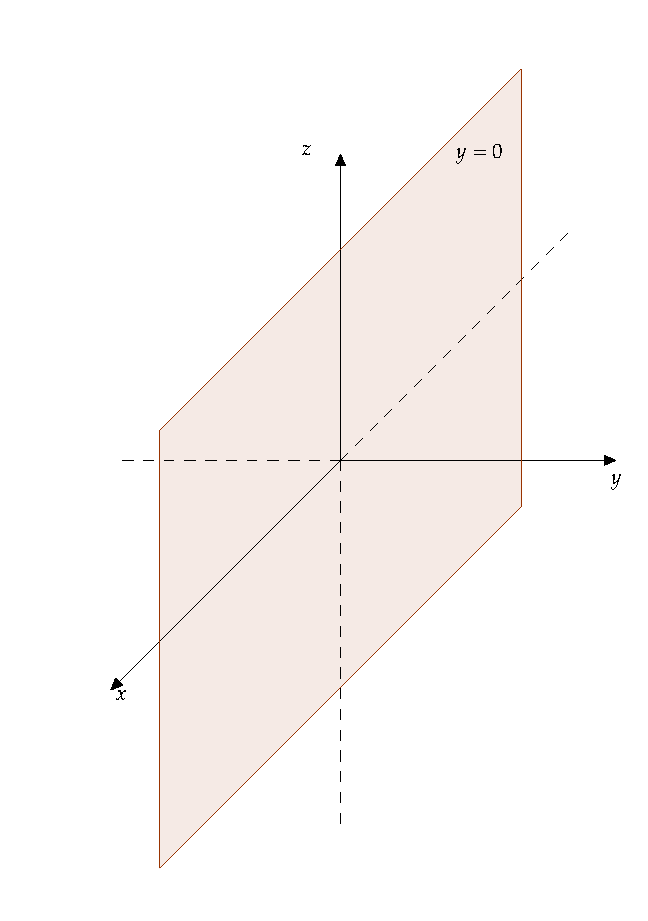
\includegraphics{plano-y=0.pdf}
                % \definecolor{zzttqq}{rgb}{0.6,0.2,0.0}
                % \begin{tikzpicture}[line cap=round,line join=round,>=triangle 45,x=1.0cm,y=1.0cm,scale=1.3]
                %     \clip(-4.3,-6.0) rectangle (4.0,6.0);
                %     \fill[color=zzttqq,fill=zzttqq,fill opacity=0.1] (-2.36,0.38000000000000017) -- (2.3550000000000004,5.095000000000001) -- (2.3550000000000004,-0.6012666666666663) -- (-2.36,-5.3162666666666665) -- cycle;
                %     \draw [->] (0.0,0.0) -- (0.0,4.0);
                %     \draw [->] (0.0,0.0) -- (3.6,0.0);
                %     \draw [->] (0.0,0.0) -- (-3.0,-3.0);
                %     \draw [dash pattern=on 5pt off 5pt] (0.0,0.0)-- (-2.84,0.0);
                %     \draw [dash pattern=on 5pt off 5pt] (0.0,0.0)-- (0.0,-4.82);
                %     \draw [dash pattern=on 5pt off 5pt] (0.0,0.0)-- (3.0,3.0);
                %     \draw [color=zzttqq] (-2.36,0.38000000000000017)-- (2.3550000000000004,5.095000000000001);
                %     \draw [color=zzttqq] (2.3550000000000004,5.095000000000001)-- (2.3550000000000004,-0.6012666666666663);
                %     \draw [color=zzttqq] (2.3550000000000004,-0.6012666666666663)-- (-2.36,-5.3162666666666665);
                %     \draw [color=zzttqq] (-2.36,-5.3162666666666665)-- (-2.36,0.38000000000000017);
                %     \draw (1.4000000000000001,4.219999999999999) node[anchor=north west] {$y = 0$};
                %     \draw (-3.02,-2.9000000000000012) node[anchor=north west] {$x$};
                %     \draw (3.42,-0.08000000000000114) node[anchor=north west] {$y$};
                %     \draw (-0.6,4.199999999999999) node[anchor=north west] {$z$};
                % \end{tikzpicture}
            \end{figure}
            Agora, se $\vec{v} = (1,0,0)$ e $P_0(0,0,0)$, ent\~ao a equa\c{c}\~ao do plano ser\'a $x = 0$.
            \begin{figure}[!h]
                \centering
                \caption{Plano $x = 0$}
                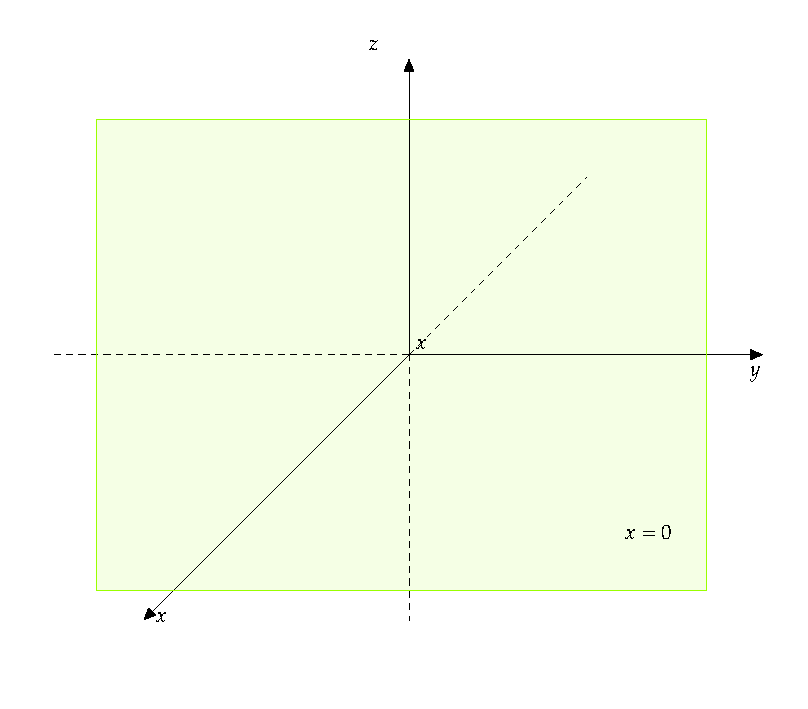
\includegraphics{plano-x=0.pdf}
                % \definecolor{zzffqq}{rgb}{0.6,1.0,0.0}
                % \begin{tikzpicture}[line cap=round,line join=round,>=triangle 45,x=1.0cm,y=1.0cm,scale=1.5]
                %     \clip(-4.5,-4.0) rectangle (4.5,4.0);
                %     \fill[color=zzffqq,fill=zzffqq,fill opacity=0.1] (-3.528888888888888,2.6497333333333333) -- (3.36,2.6497333333333333) -- (3.36,-2.66) -- (-3.528888888888888,-2.66) -- cycle;
                %     \draw [->] (0.0,0.0) -- (0.0,3.34);
                %     \draw [->] (0.0,0.0) -- (4.0,0.0);
                %     \draw [->] (0.0,0.0) -- (-3.0,-3.0);
                %     \draw [dash pattern=on 3pt off 3pt] (0.0,0.0)-- (-4.0,0.0);
                %     \draw [dash pattern=on 3pt off 3pt] (0.0,0.0)-- (0.0,-3.0);
                %     \draw [dash pattern=on 3pt off 3pt] (0.0,0.0)-- (2.0,2.0);
                %     \draw [color=zzffqq] (-3.528888888888888,2.6497333333333333)-- (3.36,2.6497333333333333);
                %     \draw [color=zzffqq] (3.36,2.6497333333333333)-- (3.36,-2.66);
                %     \draw [color=zzffqq] (3.36,-2.66)-- (-3.528888888888888,-2.66);
                %     \draw [color=zzffqq] (-3.528888888888888,-2.66)-- (-3.528888888888888,2.6497333333333333);
                %     \draw (-2.94,-2.820000000000001) node[anchor=north west] {$x$};
                %     \draw (3.7600000000000002,-0.04000000000000114) node[anchor=north west] {$y$};
                %     \draw (-0.54,3.639999999999999) node[anchor=north west] {$z$};
                %     \draw (2.36,-1.8400000000000012) node[anchor=north west] {$x = 0$};
                %     \draw (0.0,0.25999999999999884) node[anchor=north west] {$x$};
                % \end{tikzpicture}
            \end{figure}
        \end{solucao}
        \item Passando pelos pontos $A(3,1,-2)$, $B(5,2,1)$ e $C(2,0,2)$.
        \begin{solucao}
            Sejam
            \begin{align*}
                \vec{u} = \vec{AB} = (2,1,3)\\
                \vec{v} = \vec{AC} = (-1,-1,4).
            \end{align*}
            Um vetor normal ao plano \'e dado por $\vec{w} = \vec{u}\times\vec{v}$. Assim
            \[
                \vec{w} = \det \begin{bmatrix}
                    \vec{i} & \vec{j} & \vec{k}\\
                    2 & 1 & 3\\
                    -1 & -1 & 4
                \end{bmatrix} = 4\vec{i} - 3\vec{j} - 2\vec{k} + \vec{k} + 3\vec{i} - 8\vec{j}.
            \]
            Assim $\vec{w} = (7,-11,-1)$ e portanto a equa\c{c}\~ao do plano \'e
            \[
                7x - 11y - z - 12 = 0.
            \]
        \end{solucao}
    \end{enumerate}
\end{exemplos}

Dada uma equa\c{c}\~ao da forma
    \[
        ax + by + cz + d = 0,
    \]
onde $a$, $b$ e $c$ n\~ao s\~ao simultaneamente nulos, existe um plano $\pi$ representado por esta equa\c{c}\~ao? A resposta \'e afirmativa. Suponha que $a \ne 0$. Tome $\vec{v} = (a,b,c) \ne 0$ e $P_0(-d/a,0,0)$. A equa\c{c}\~ao do plano com vetor normal $\vec{v}$ e passando por $P_0$ \'e dada por
    \begin{align*}
        &\vec{P_0P}\cdot\vec{v} = 0\\
        &\left(x + \dfrac{d}{a},y,z\right)\cdot(a,b,c) = 0\\
        &ax + by + cz + d = 0.
    \end{align*}
Portanto qualquer equa\c{c}\~ao da forma $ax + by + cz + d = 0$, com $a$, $b$ e $c$ n\~ao simultaneamente nulos define um plano.

Sejam $\pi_1$ e $\pi_2$ dois planos dados por
    \begin{align*}
        \pi_1 : a_1x + b_1y + c_1z + d_1 = 0\\
        \pi_2 : a_2x + b_2y + c_2z + d_2 = 0.
    \end{align*}
onde os vetores normais de $\pi_1$ e $\pi_2$ s\~ao, respectivamente,
    \begin{align*}
        \vec{v_1} = (a_1, b_1, c_1)\\
        \vec{v_2} = (a_2, b_2, c_2).
    \end{align*}
Os planos $\pi_1$ e $\pi_2$ s\~ao \textbf{paralelos} se, e somente se, $\vec{v_1} \varparallel\vec{v_2}$. Para que $\pi_1$ e $\pi_2$ sejam iguais devemos ter $\vec{v_1}\varparallel\vec{v_2}$  e dados $P_1\in\pi_1$ e $P_2\in\pi_2$ o vetor $\vec{P_1P_2}$ deve ser tal que $\vec{P_1P_2}\perp\vec{v_1}$ ou $\vec{P_1P_2}\perp\vec{v_2}$.

\begin{exemplo}
    Dados os seguintes planos, determinar quais s\~ao iguais ou paralelos dois a dois:
    \begin{center}
        \begin{tabular}{cc}
            $\pi_1 : 2x - y + 3z = 0$ & 
            $\pi_2 : x - y - 3 = 0$\\
            $\pi_3 : y - 2x - 3z = 2$ & $\pi_4 : 2x - 2y = 6$\\
            $\pi_5 : x = 0$.
        \end{tabular}
    \end{center}
    \begin{solucao}
        Os vetores normais a cada plano s\~ao
        \begin{center}
            \begin{tabular}{cc}
                $\vec{v_1} = (2, -1, 3)$ & $\vec{v_2} = (1,-1,0)$\\
                $\vec{v_3} = (-2, 1, -3)$ & $\vec{v_2} = (2,-2,0)$\\
                $\vec{v_5} = (1, 0, 0)$.
            \end{tabular}
        \end{center}
        Como $\vec{v_1} = -\vec{v_3}$ ent\~ao $\vec{v_1}\varparallel\vec{v_2}$. Agora $P_1(0,0,0)\in\pi_1$ e $P_2(0,2,0)\in\pi_3$. Da{\'\i}
        \[
            \vec{P_1P_2}\cdot\vec{v_1} = (0,2,0)\cdot(2,-1,3) = -2 \ne 0.
        \]
        Logo $\pi_1$ e $\pi_3$ s\~ao paralelos e distintos.
        Agora, como $\vec{v_4} = 2\vec{v_2}$ ent\~ao $\vec{v_2}\varparallel\vec{v_4}$. Mas $P_1(3,0,0)\in\pi_2$ e $P_2(0,-3,0)\in\pi_4$. Da{\'\i}
        \[
            \vec{P_1P_2}\cdot\vec{v_2} = (-3,-3,0)\cdot(1,-1,0) = 0.
        \]
        Logo $\pi_2 =\pi_4$.

        Os demais planos n\~ao s\~ao paralelos.
    \end{solucao}
\end{exemplo}

% section equacoes_do_plano (end)

\section{Equa\c{c}\~oes da Reta} % (fold)
\label{sec:equacoes_da_reta}

Seja $\vec{v}$ um vetor e $A$ um ponto. Sabemos que a reta $r$ passando por $A$ e paralela ao vetor $\vec{v}$ tem equa\c{c}\~ao
\begin{equation}
    \vec{AP} = t\vec{v}
\end{equation}
onte $t \in \real$ e $P$ \'e um ponto qualquer de $r$. Sendo $A$ um ponto em $\real^3$ e $\vec{v}$ um vetor de $\real^3$ temos
\begin{align*}
    A = (x_0, y_0, z_0)\\
    \vec{v} = (a, b, c).
\end{align*}
Da{\'\i} um ponto $P(x, y, z)$ pertence \`a reta $r$ se, e somente se,
\[
    \vec{AP} = (x - x_0, y - y_0, z - z_0) = t(a, b, c).
\]
Logo $P(x, y, z)$ pertence \`a reta $r$, se e s\'o se, $P(x,y,z)$ satisfaz as equa\c{c}\~oes
\begin{equation}\label{equacoesparametricasretaespaco}
    \begin{cases}
        x = x_0 + ta\\
        y = y_0 + tb\\
        z = z_0 + tc
    \end{cases}; \quad t \in \real.
\end{equation}
Tais equa\c{c}\~oes s\~ao chamadas de \textbf{equa\c{c}\~oes param\'etricas} da reta $r$. O vetor $\vec{v}$ \'e chamado de \textbf{vetor diretor} de $r$.\index{Reta!Equa\c{c}\~oes Param\'etricas}\index{Reta!Vetor Diretor}

\begin{exemplo}
    As equa\c{c}\~oes param\'etricas da reta $r$ passando por $P_0(-3,3/2,4)$ e paralela ao vetor $\vec{v} = (-6,1,4)$ s\~ao
    \[
        \begin{cases}
            x = -3 - 6t\\
            y = 3/2 + t\\
            z = 4 + 4t
        \end{cases},\quad t \in \real.
    \]
\end{exemplo}

De forma an\'aloga ao casa do plano, se $\vec{v} = (a,b,c)$ \'e tal que $abc \ne 0$, ent\~ao podemos reescrever \eqref{equacoesparametricasretaespaco} como
\[
    \dfrac{x - x_0}{a} = \dfrac{y - y_0}{b} = \dfrac{z - z_0}{c}
\]
que s\~ao chamadas de \textbf{equa\c{c}\~oes na forma sim\'etrica} da reta $r$.\index{Reta!Equa\c{c}\~oes Sim\'etricas}
% section equacoes_da_reta (end)
\section{Interse\c{c}\~oes} % (fold)
\label{sec:intersecoes}
\subsection{Entre retas} % (fold)
\label{sub:entre_retas}
Considere duas retas $r$ e $s$ de equa\c{c}\~oes
\[
    r: \begin{cases}
        x = x_0 + ta\\
        y = y_0 + tb\\
        z = z_0 + tc
    \end{cases}; \quad s: \begin{cases}
        x = x_1 + sd\\
        y = y_1 + se\\
        z = z_1 + sf
    \end{cases}; t,\ s \in \real.
\]
Os vetores diretores de $r$ e $s$ s\~ao $\vec{u} = (a,b,c)$ e $\vec{v} = (d,e,f)$ respectivamente.
\begin{enumerate}
\item Se $\vec{u}\varparallel\vec{v}$, ent\~ao $r$ e $s$ s\~ao paralelas ou coincidentes. Elas ser\~ao coincidentes se, e somente se, possuirem algum ponto em comum.\index{Retas!Paralelas}
\begin{figure}[h]
    \centering
    \caption{Retas Paralelas}
    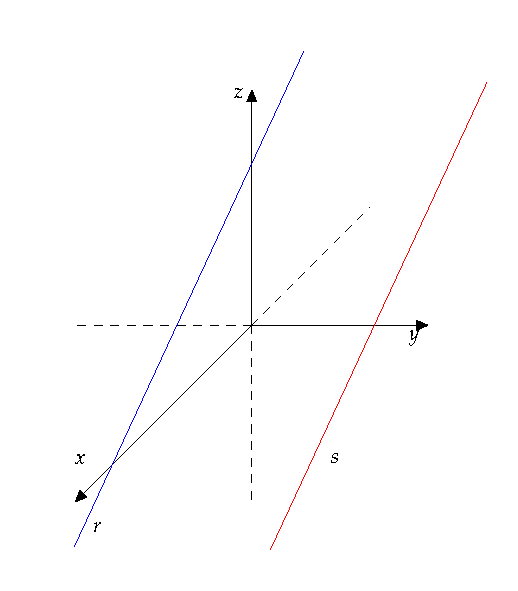
\includegraphics{retas-paralelas-espaco.pdf}
    % \definecolor{ffqqqq}{rgb}{1,0,0}
    % \definecolor{qqqqff}{rgb}{0,0,1}
    % \begin{tikzpicture}[line cap=round,line join=round,>=triangle 45,x=1.0cm,y=1.0cm]
    %     \clip(1,-4.5) rectangle (9.5,5.5);
    %     \draw [->] (5,0) -- (5,4);
    %     \draw [->] (5,0) -- (8,0);
    %     \draw [->] (5,0) -- (2,-3);
    %     \draw [dash pattern=on 4pt off 4pt] (5,0)-- (2,0);
    %     \draw [dash pattern=on 4pt off 4pt] (5,0)-- (5,-3);
    %     \draw [dash pattern=on 4pt off 4pt] (5,0)-- (7,2);
    %     \draw [color=qqqqff] (1.99,-3.76)-- (5.88,4.64);
    %     \draw (2.18,-3.2) node[anchor=north west] {$r$};
    %     \draw (1.88,-2.06) node[anchor=north west] {$x$};
    %     \draw (7.52,0.04) node[anchor=north west] {$y$};
    %     \draw (4.58,4.14) node[anchor=north west] {$z$};
    %     \draw (6.22,-2.04) node[anchor=north west] {$s$};
    %     \draw [color=ffqqqq] (5.31,-3.81)-- (8.98,4.11);
    % \end{tikzpicture}
\end{figure}
\item Se os vetores diretores n\~ao s\~ao paralelos, temos duas possibilidades. Considere os pontos $P_0(x_0,y_0,z_0) \in r$ e $P_1(x_1,y_1,z_1) \in s$.
\begin{enumerate}
\item Se $\vec{P_1P_2}$, $\vec{u}$ e $\vec{v}$ est\~ao no mesmo plano, isto \'e, $\vec{P_1P_2}\cdot(\vec{u}\times\vec{v}) = 0$ ent\~ao $r$ e $s$ s\~ao concorrentes.\index{Retas!Concorrentes}
\begin{figure}[h]
    \centering
    \caption{Retas Concorrentes}
    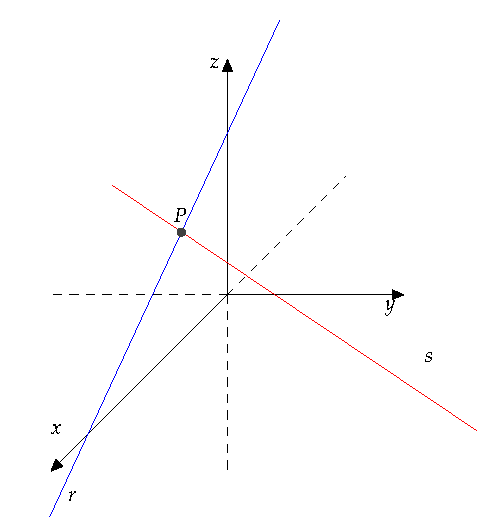
\includegraphics{retas-concorrentes-espaco.pdf}
    % \definecolor{uququq}{rgb}{0.25,0.25,0.25}
    % \definecolor{ffqqqq}{rgb}{1,0,0}
    % \definecolor{qqqqff}{rgb}{0,0,1}
    % \begin{tikzpicture}[line cap=round,line join=round,>=triangle 45,x=1.0cm,y=1.0cm]
    %     \clip(1.5,-4) rectangle (9.5,5);
    %     \draw [->] (5,0) -- (5,4);
    %     \draw [->] (5,0) -- (8,0);
    %     \draw [->] (5,0) -- (2,-3);
    %     \draw [dash pattern=on 4pt off 4pt] (5,0)-- (2,0);
    %     \draw [dash pattern=on 4pt off 4pt] (5,0)-- (5,-3);
    %     \draw [dash pattern=on 4pt off 4pt] (5,0)-- (7,2);
    %     \draw [color=qqqqff] (1.99,-3.76)-- (5.88,4.64);
    %     \draw (2.18,-3.2) node[anchor=north west] {$r$};
    %     \draw (1.88,-2.06) node[anchor=north west] {$x$};
    %     \draw (7.52,0.04) node[anchor=north west] {$y$};
    %     \draw (4.58,4.14) node[anchor=north west] {$z$};
    %     \draw (8.22,-0.84) node[anchor=north west] {$s$};
    %     \draw [color=ffqqqq] (3.04,1.86)-- (9.22,-2.3);
    %     \fill [color=uququq] (4.22,1.06) circle (2.0pt);
    %     \draw (4.2,1.36) node {$P$};
    % \end{tikzpicture}
\end{figure}
\item Se $\vec{P_1P_2}$, $\vec{u}$ e $\vec{v}$ est\~ao planos diferentes, isto \'e, $\vec{P_1P_2}\cdot(\vec{u}\times\vec{v}) \ne 0$ ent\~ao $r$ e $s$ s\~ao chamadas de  \textbf{retas reversas}.\index{Retas! Reversas}
\begin{figure}[h]
   \centering
   \caption{Retas Reversas}
   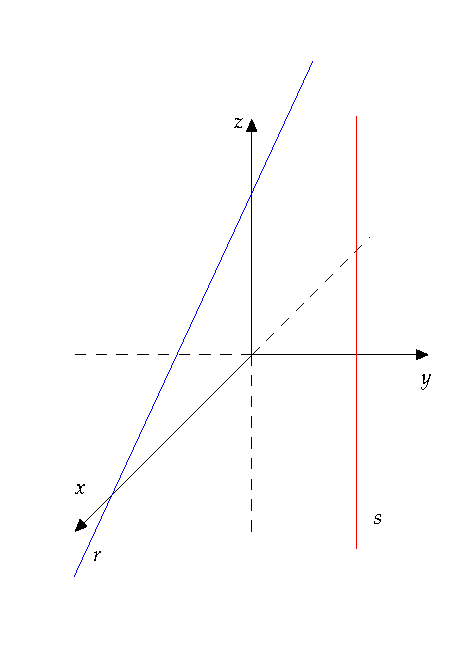
\includegraphics{retas-reversas-espaco.pdf}
   % \definecolor{ffqqqq}{rgb}{1,0,0}
   %  \definecolor{qqqqff}{rgb}{0,0,1}
   %  \begin{tikzpicture}[line cap=round,line join=round,>=triangle 45,x=1.0cm,y=1.0cm]
   %      \clip(1,-5) rectangle (8.5,6);
   %      \draw [->] (5,0) -- (5,4);
   %      \draw [->] (5,0) -- (8,0);
   %      \draw [->] (5,0) -- (2,-3);
   %      \draw [dash pattern=on 5pt off 5pt] (5,0)-- (2,0);
   %      \draw [dash pattern=on 5pt off 5pt] (5,0)-- (5,-3);
   %      \draw [dash pattern=on 5pt off 5pt] (5,0)-- (7,2);
   %      \draw [color=qqqqff] (1.99,-3.76)-- (6.03,4.96);
   %      \draw [color=ffqqqq] (6.78,4.04)-- (6.78,-3.28);
   %      \draw (2.18,-3.2) node[anchor=north west] {$r$};
   %      \draw (1.88,-2.06) node[anchor=north west] {$x$};
   %      \draw (7.72,-0.2) node[anchor=north west] {$y$};
   %      \draw (4.58,4.14) node[anchor=north west] {$z$};
   %      \draw (6.94,-2.58) node[anchor=north west] {$s$};
   %  \end{tikzpicture}
\end{figure}
\end{enumerate} 
\end{enumerate}

\begin{exemplos}
    Determine se os seguintes pares de retas s\~ao paralelas, concorrentes ou reversas:
    \begin{enumerate}
        \item $r: \dfrac{x - 2}{2} = y + 3 = \dfrac{z - 2}{3}$; $s:\dfrac{x}{4} = \dfrac{y+3}{2} = \dfrac{z-2}{6}$
        \begin{solucao}
            Como $\vec{u} = (2,1,3)$ e $\vec{v} = (4,2,6)$ s\~ao vetores diretores de $r$ e $s$ respectivamente, ent\~ao $\vec{u}\varparallel\vec{v}$. Mas $P_0(0,-3,2)\in s$ e $P_0\notin r$, logo $r$ e $s$ s\~ao paralelas e distintas.
        \end{solucao}
        \item 
        \[
            r: \begin{cases}
                x = 1 + 2t\\
                y = 1 + 2t\\
                z = 1 + t
            \end{cases},\quad s: \begin{cases}
                x = s\\
                y = s\\
                z = 0
            \end{cases}
        \]
        \begin{solucao}
            Como $\vec{u} = (2,2,1)$ e $\vec{v} = (1,1,0)$ s\~ao vetores diretores de $r$ e $s$ respectivamente, ent\~ao $r$ e $s$ s\~ao concorrentes ou reversas. Igualando as equa\c{c}\~oes de $r$ e $s$ obtemos
            \begin{align*}
                1 + 2t = s\\
                1 + 2t = s\\
                1 + t = 0
            \end{align*}
            donde $t = -1$ e $s = -1$. Portanto $r$ e $s$ s\~ao concorrentes e o ponto de interse\c{c}\~ao \'e $P(-1,-1,0)$.
        \end{solucao}
        \item
        \[
            r: \begin{cases}
                x = 1 + 2t\\
                y = 2 + t\\
                z = -1 + 2t
            \end{cases},\quad s: \begin{cases}
                x = 2 + s\\
                y = 1 + s\\
                z = -1 + 2s
            \end{cases}
        \]
        \begin{solucao}
            Como $\vec{u} = (2,1,2)$ e $\vec{v} = (1,1,2)$ s\~ao vetores diretores de $r$ e $s$ respectivamente, ent\~ao $r$ e $s$ s\~ao concorrentes ou paralelas. Igualando as equa\c{c}\~oes de $r$ e $s$ obtemos
            \begin{equation}\label{exemploretasreversas}
                \begin{cases}
                    1 + 2t = 2 + s\\
                    2 + t = 1 + s\\
                    -1 + 2t = -1 + 2s    
                \end{cases}
            \end{equation}
            Da primeira e segunda equa\c{c}\~ao obtemos o sistema
            \[
                \begin{cases}
                    2t - s = 1\\
                    t - s = -1
                \end{cases}
            \]
            Cuja solu\c{c}\~ao \'e $t = 2$ e $s = 3$. Substituinto esse valores na terceira equa\c{c}\~ao de \eqref{exemploretasreversas} obtemos $3 \ne 5$. Portanto $r$ e $s$ s\~ao reversas.
        \end{solucao}
    \end{enumerate}
\end{exemplos}
% subsection entre_retas (end)

\subsection{Entre planos} % (fold)
\label{sub:entre_planos}
Dados tr\^es planos $\pi_1$, $\pi_2$ e $\pi_3$ de equa\c{c}\~oes
\begin{align*}
    \pi_1 : a_1x + b_1y + c_1z + d_1 = 0\\
    \pi_2 : a_2x + b_2y + c_2z + d_2 = 0\\
    \pi_3 : a_3x + b_3y + c_3z + d_3 = 0.
\end{align*}
A interse\c{c}\~ao entre eles ser\'a constitu{\'\i}da pelos pontos cujas coordenadas sejam as solu\c{c}\~oes do sistema forma pelas equa\c{c}\~oes de $\pi_1$, $\pi_2$ e $\pi_3$ simultaneamente, ou seja, devem ser solu\c{c}\~oes do sistema
\[
    \begin{cases}
        a_1x + b_1y + c_1z + d_1 = 0\\
        a_2x + b_2y + c_2z + d_2 = 0\\
        a_3x + b_3y + c_3z + d_3 = 0.
    \end{cases}
\]

\begin{figure}[h]
    \centering
    \caption{$\pi_1\cap\pi_2\cap\pi_3 = \{P\}$}
    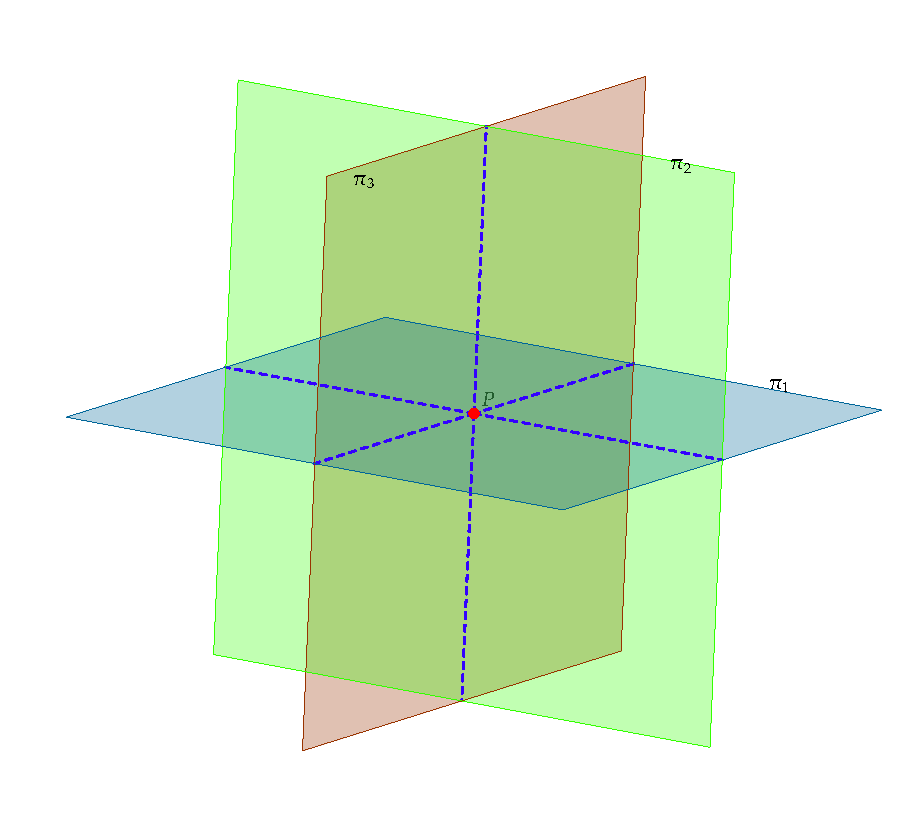
\includegraphics{intersecao-tres-planos.pdf}
    % \definecolor{qqwwzz}{rgb}{0,0.4,0.6}
    % \definecolor{ttffqq}{rgb}{0.2,1,0}
    % \definecolor{zzttqq}{rgb}{0.6,0.2,0}
    % \definecolor{ttqqff}{rgb}{0.2,0,1}
    % \definecolor{ffqqqq}{rgb}{1,0,0}
    % \begin{tikzpicture}[line cap=round,line join=round,>=triangle 45,x=1.0cm,y=1.0cm,scale=0.5]
    %     \coordinate[label=$P$] (P) at (0.5,0);
    %     \clip(-15,-14) rectangle (15,14);
    %     \fill[color=zzttqq,fill=zzttqq,fill opacity=0.1] (-5.81,-11.42) -- (-4.98,8.04) -- (5.81,11.42) -- (4.98,-8.04) -- cycle;
    %     \fill[color=ttffqq,fill=ttffqq,fill opacity=0.1] (-7.99,11.3) -- (-8.82,-8.16) -- (7.99,-11.3) -- (8.82,8.16) -- cycle;
    %     \fill[color=qqwwzz,fill=qqwwzz,fill opacity=0.1] (-13.81,-0.12) -- (3.01,-3.26) -- (13.81,0.12) -- (-3.01,3.26) -- cycle;
    %     \draw [dashed,line width=1pt,color=ttqqff] (0,0) -- (-5.4,-1.69);
    %     \draw [dashed,line width=1pt,color=ttqqff] (0,0) -- (8.41,-1.57);
    %     \draw [dashed,line width=1pt,color=ttqqff] (0,0) -- (0.42,9.73);
    %     \draw [dashed,line width=1pt,color=ttqqff] (5.4,1.69)-- (0,0);
    %     \draw [dashed,line width=1pt,color=ttqqff] (0,0)-- (-8.41,1.57);
    %     \draw [dashed,line width=1pt,color=ttqqff] (0,0)-- (-0.42,-9.73);
    %     \draw [color=zzttqq] (-5.81,-11.42)-- (-4.98,8.04);
    %     \draw [color=zzttqq] (-4.98,8.04)-- (5.81,11.42);
    %     \draw [color=zzttqq] (5.81,11.42)-- (4.98,-8.04);
    %     \draw [color=zzttqq] (4.98,-8.04)-- (-5.81,-11.42);
    %     \draw [color=ttffqq] (-7.99,11.3)-- (-8.82,-8.16);
    %     \draw [color=ttffqq] (-8.82,-8.16)-- (7.99,-11.3);
    %     \draw [color=ttffqq] (7.99,-11.3)-- (8.82,8.16);
    %     \draw [color=ttffqq] (8.82,8.16)-- (-7.99,11.3);
    %     \draw [color=qqwwzz] (-13.81,-0.12)-- (3.01,-3.26);
    %     \draw [color=qqwwzz] (3.01,-3.26)-- (13.81,0.12);
    %     \draw [color=qqwwzz] (13.81,0.12)-- (-3.01,3.26);
    %     \draw [color=qqwwzz] (-3.01,3.26)-- (-13.81,-0.12);
    %     \draw (9.73,1.43) node[anchor=north west] {$\pi_1$};
    %     \draw (6.4,8.85) node[anchor=north west] {$\pi_2$};
    %     \draw (-4.35,8.31) node[anchor=north west] {$\pi_3$};
    %     \fill [color=ffqqqq] (0,0) circle (5pt);
    % \end{tikzpicture}
\end{figure}

\begin{figure}[h]
    \caption{$\pi_1\cap\pi_2\cap\pi_3 = \emptyset$}
    \centering
    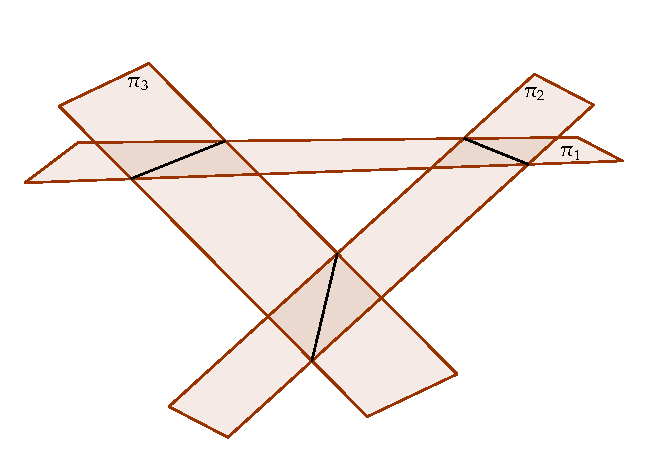
\includegraphics{intersecao-tres-planos-dois-a-dois.pdf}
    % \definecolor{zzttqq}{rgb}{0.6,0.2,0}
    % \begin{tikzpicture}[line cap=round,line join=round,>=triangle 45,x=1.0cm,y=1.0cm]
    %     \clip(0,-5) rectangle (12,2);
    %     \fill[color=zzttqq,fill=zzttqq,fill opacity=0.1] (1.38,0.86) -- (1.94,1.58) -- (7.32,-3.94) -- (6.76,-4.66) -- cycle;
    %     \fill[color=zzttqq,fill=zzttqq,fill opacity=0.1] (4.6,-4.3) -- (10.74,0.86) -- (8.62,1.12) -- (2.48,-4.04) -- cycle;
    %     \fill[color=zzttqq,fill=zzttqq,fill opacity=0.1] (0.56,-0.16) -- (0.62,-0.84) -- (11.62,-0.52) -- (10.48,0.12) -- cycle;
    %     \draw [color=zzttqq] (1.38,0.86)-- (1.94,1.58);
    %     \draw [color=zzttqq] (1.94,1.58)-- (7.32,-3.94);
    %     \draw [color=zzttqq] (7.32,-3.94)-- (6.76,-4.66);
    %     \draw [color=zzttqq] (6.76,-4.66)-- (1.38,0.86);
    %     \draw [color=zzttqq] (4.6,-4.3)-- (10.74,0.86);
    %     \draw [color=zzttqq] (10.74,0.86)-- (8.62,1.12);
    %     \draw [color=zzttqq] (8.62,1.12)-- (2.48,-4.04);
    %     \draw [color=zzttqq] (2.48,-4.04)-- (4.6,-4.3);
    %     \draw (5.59,-3.46)-- (5.19,-1.76);
    %     \draw [color=zzttqq] (0.56,-0.16)-- (0.62,-0.84);
    %     \draw [color=zzttqq] (0.62,-0.84)-- (11.62,-0.52);
    %     \draw [color=zzttqq] (11.62,-0.52)-- (10.48,0.12);
    %     \draw [color=zzttqq] (10.48,0.12)-- (0.56,-0.16);
    %     \draw (3.55,-0.08)-- (2.97,-0.77);
    %     \draw (7.32,0.03)-- (9.01,-0.6);
    %     \draw (10.56,0.12) node[anchor=north west] {$\pi_1$};
    %     \draw (9.52,1.02) node[anchor=north west] {$\pi_2$};
    %     \draw (1.84,1.38) node[anchor=north west] {$\pi_3$};
    % \end{tikzpicture}
\end{figure}

\begin{figure}[h]
    \centering
    \caption{$\pi_1\cap\pi_2\cap\pi_3 = \emptyset$}
    {\centering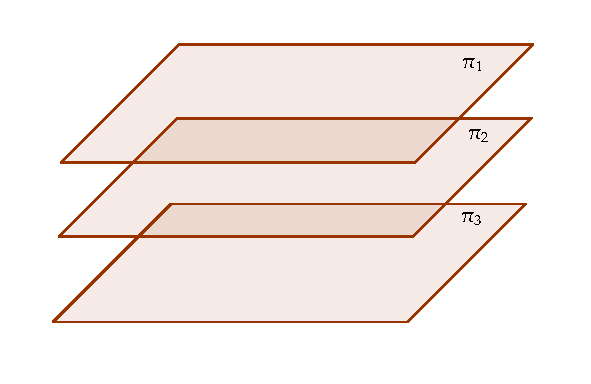
\includegraphics{tres-planos-paralelos.pdf}}
    % \definecolor{zzttqq}{rgb}{0.6,0.2,0}
    % \begin{tikzpicture}[line cap=round,line join=round,>=triangle 45,x=1.0cm,y=1.0cm]
    %     \clip(-5,-5) rectangle (7.5,7);
    %     \fill[color=zzttqq,fill=zzttqq,fill opacity=0.1] (0,6) -- (-2,4.02) -- (5.55,4.02) -- (7.1,6) -- cycle;
    %     \fill[color=zzttqq,fill=zzttqq,fill opacity=0.1] (-1.86,2.01) -- (-3.65,0) -- (5.02,0) -- (6.52,2.01) -- cycle;
    %     \fill[color=zzttqq,fill=zzttqq,fill opacity=0.1] (-2.65,-2) -- (-4.5,-4.01) -- (4.51,-4.02) -- (6,-2) -- cycle;
    %     \draw [color=zzttqq] (0,6)-- (-2,4.02);
    %     \draw [color=zzttqq] (-2,4.02)-- (5.55,4.02);
    %     \draw [color=zzttqq] (5.55,4.02)-- (7.1,6);
    %     \draw [color=zzttqq] (7.1,6)-- (0,6);
    %     \draw [color=zzttqq] (-1.86,2.01)-- (-3.65,0);
    %     \draw [color=zzttqq] (-3.65,0)-- (5.02,0);
    %     \draw [color=zzttqq] (5.02,0)-- (6.52,2.01);
    %     \draw [color=zzttqq] (6.52,2.01)-- (-1.86,2.01);
    %     \draw [color=zzttqq] (-2.65,-2)-- (-4.5,-4.01);
    %     \draw [color=zzttqq] (-4.5,-4.01)-- (4.51,-4.02);
    %     \draw [color=zzttqq] (4.51,-4.02)-- (6,-2);
    %     \draw [color=zzttqq] (6,-2)-- (-2.65,-2);
    %     \draw (5.77,6.1) node[anchor=north west] {$\pi_1$};
    %     \draw (5.21,2.01) node[anchor=north west] {$\pi_2$};
    %     \draw (4.73,-1.93) node[anchor=north west] {$\pi_3$};
    % \end{tikzpicture}
\end{figure}
\begin{exemplos}
    Encontre a interse\c{c}\~ao entre os planos:
    \begin{enumerate}
        \item $\pi_1 : x = y$, $\pi_2 : 2x - z = 0$ e $\pi_3 : 3x + 2y + z + 3 = 0$
        \begin{solucao}
            A interse\c{c}\~ao ser\'a dada pela solu\c{c}\~ao do sistema
            \[
                \begin{cases}
                    x - y = 0\\
                    2x - z = 0\\
                    3x + 2y + z + 3 = 0.
                \end{cases}
            \]
            Resolvendo tal sistema obtemos que $\pi_1\cap\pi_2\cap\pi_3 = \{(-3/7,-3/7,-6/7)\}$.
        \end{solucao}
        \item $\pi_1 : 2x + y = 1$, $\pi_2 : x - y + z = 0$
        \begin{solucao}
            A interse\c{c}\~ao ser\'a dada pela solu\c{c}\~ao do sistema
            \[
                \begin{cases}
                    2x + y = 1\\
                    x - y + z = 0.
                \end{cases}
            \]
            Resolvendo tal sistema obtemos $z = 1 - 3x$ e $y = 1 - 2x$. Logo
            \[
                \pi_1\cap\pi_2 = \{(x,1 - 2x,1 - 3x) \mid x \in \real\}.
            \]
            Fazendo $x = t$ podemos escrever
            \[
                \begin{cases}
                    x = t\\
                    y = 1 - 2t\\
                    z = 1 - 3t
                \end{cases}; t \in \real
            \]
            que \'e a equa\c{c}\~ao de uma reta passando pelo ponto $P_0(0,1,1)$ e com vetor diretor $\vec{v} = (1,-2,-3)$.
        \end{solucao}
    \end{enumerate}
\end{exemplos}

% subsection entre_planos (end)

\subsection{Entre retas e planos} % (fold)
\label{sub:entre_retas_e_planos}

Para encontrar a interse\c{c}\~ao de uma reta $r$ com um plano $\pi$, basta resolver o sistema formado pelas equa\c{c}\~oes de $r$ e de $\pi$. Se o sistema tiver uma \'unica solu\c{c}\~ao $P_0(x_0, y_0, z_0)$, ent\~ao $r \cap \pi = \{P_0\}$. Se o sistema for indeterminado ent\~ao $r\subset \pi$ e se o sistema for imposs{\'\i}vel ent\~ao $r\cap\pi = \emptyset$ e $r \varparallel \pi$.
\begin{figure}[h]
    \centering
    \caption{$r\cap\pi = \{P_0\}$}
    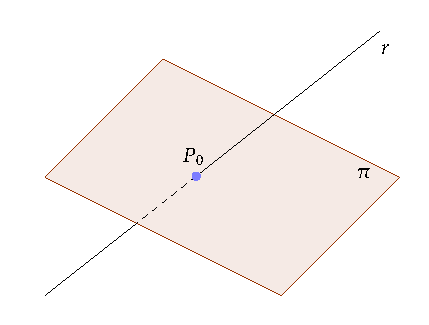
\includegraphics{intersecao-reta-plano.pdf}
    % \definecolor{xdxdff}{rgb}{0.49,0.49,1}
    % \definecolor{zzttqq}{rgb}{0.6,0.2,0}
    % \begin{tikzpicture}[line cap=round,line join=round,>=triangle 45,x=1.0cm,y=1.0cm]
    %     \clip(3.5,-2.5) rectangle (10.5,3);
    %     \fill[color=zzttqq,fill=zzttqq,fill opacity=0.1] (6,2) -- (4,0) -- (8,-2) -- (10,0) -- cycle;
    %     \draw [color=zzttqq] (6,2)-- (4,0);
    %     \draw [color=zzttqq] (4,0)-- (8,-2);
    %     \draw [color=zzttqq] (8,-2)-- (10,0);
    %     \draw [color=zzttqq] (10,0)-- (6,2);
    %     \draw (6.56,0.02)-- (9.66,2.47);
    %     \draw [dashed] (6.56,0.02)-- (5.55,-0.78);
    %     \draw (5.55,-0.78)-- (4,-2);
    %     \draw (9.16,0.28) node[anchor=north west] {$\pi$};
    %     \draw (9.56,2.38) node[anchor=north west] {$r$};
    %     \fill [color=xdxdff] (6.56,0.02) circle (2pt);
    %     \draw(6.52,0.36) node {$P_0$};
    % \end{tikzpicture}
\end{figure}

\begin{figure}[h]
    \centering
    \caption{$r\cap\pi= \emptyset$}
    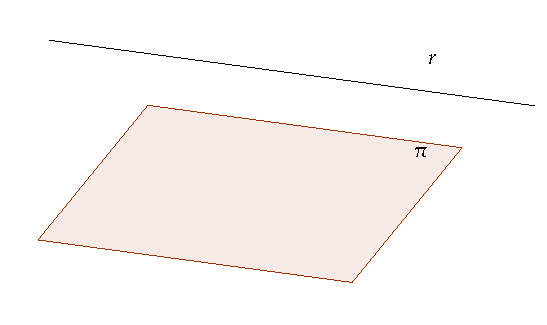
\includegraphics{intersecao-reta-plano-vazia.pdf}
    % \definecolor{zzttqq}{rgb}{0.6,0.2,0}
    % \begin{tikzpicture}[line cap=round,line join=round,>=triangle 45,x=1.0cm,y=1.0cm]
    %     \clip(4,-1) rectangle (13,4.5);
    %     \fill[color=zzttqq,fill=zzttqq,fill opacity=0.1] (6.24,2.72) -- (4.38,0.44) -- (9.7,-0.28) -- (11.56,2) -- cycle;
    %     \draw [color=zzttqq] (6.24,2.72)-- (4.38,0.44);
    %     \draw [color=zzttqq] (4.38,0.44)-- (9.7,-0.28);
    %     \draw [color=zzttqq] (9.7,-0.28)-- (11.56,2);
    %     \draw [color=zzttqq] (11.56,2)-- (6.24,2.72);
    %     \draw (10.62,2.14) node[anchor=north west] {$\pi$};
    %     \draw (10.86,3.72) node[anchor=north west] {$r$};
    %     \draw (4.58,3.82)-- (12.8,2.71);
    % \end{tikzpicture}
\end{figure}

\begin{figure}[h]
    \centering
    \caption{$r \subset \pi$}
    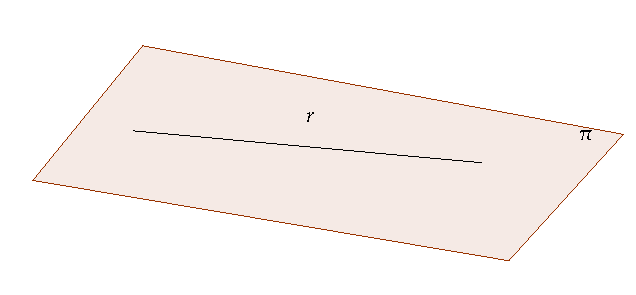
\includegraphics{reta-contida-no-plano.pdf}
    % \definecolor{zzttqq}{rgb}{0.6,0.2,0}
    % \begin{tikzpicture}[line cap=round,line join=round,>=triangle 45,x=1.0cm,y=1.0cm]
    %     \clip(4,-1.5) rectangle (14.6,3.5);
    %     \fill[color=zzttqq,fill=zzttqq,fill opacity=0.1] (6.24,2.72) -- (4.38,0.44) -- (12.44,-0.92) -- (14.38,1.22) -- cycle;
    %     \draw [color=zzttqq] (6.24,2.72)-- (4.38,0.44);
    %     \draw [color=zzttqq] (4.38,0.44)-- (12.44,-0.92);
    %     \draw [color=zzttqq] (12.44,-0.92)-- (14.38,1.22);
    %     \draw [color=zzttqq] (14.38,1.22)-- (6.24,2.72);
    %     \draw (13.5,1.42) node[anchor=north west] {$\pi$};
    %     \draw (8.88,1.72) node[anchor=north west] {$r$};
    %     \draw (6.08,1.28)-- (11.98,0.74);
    % \end{tikzpicture}
\end{figure}

\begin{exemplos}
    Encontre a interse\c{c}\~ao entre a reta $r$ e o plano $\pi$ nos seguintes casos:
    \begin{enumerate}
        \item $r: x = t + 1$, $y = 1$, $z = 1$ e $\pi : 2x - y = 3$.
        \begin{solucao}
            Substituindo as equa\c{c}\~oes da reta na do plano obtemos $t = 1$. Logo $r\cap\pi = \{(2,1,1)\}$.
        \end{solucao}
        \item
        \[
            r: \begin{cases}
                2x - y + z = 0\\
                x + y = 1
            \end{cases};
        \]
        $\pi : x - 2y + z = 5$.
        \begin{solucao}
            O sistema
            \[
                \begin{cases}
                    2x - y + z = 0\\
                    x + y = 1\\
                    x - 2y + z = 5
                \end{cases}
            \]
            n\~ao tem solu\c{c}\~ao. Logo $r\cap\pi = \emptyset$.
        \end{solucao}
        \item
        \[
            r: \begin{cases}
                2x - y + z = 0\\
                x + y = 1
            \end{cases};
        \]
        $\pi : x - y + 3z = -1$.
        \begin{solucao}
            O sistema
            \[
                \begin{cases}
                    2x - y + z = 0\\
                    x + y = 1\\
                    x - y + 3z = -1
                \end{cases}
            \]
            tem solu\c{c}\~ao dada por $x = -1 + 3z$ e $y = -2 + 6z$. Logo 
            \[
            r\cap\pi : \begin{cases}
                x = -1 + 3t\\
                y = -2 + 6t\\
                z = t
            \end{cases},
            \]
            ou seja, $r \subset \pi$.
        \end{solucao}
    \end{enumerate}
\end{exemplos}

% subsection entre_retas_e_planos (end)

% section intersecoes (end)


\section{Dist\^ancias} % (fold)
\label{sec:distancias}
\subsection{Entre ponto e plano} % (fold)
\label{sub:entre_ponto_e_plano}
Seja $P_1(x_1,y_1,z_1)$ um ponto e $\pi$ um plano de equa\c{c}\~ao $ax + by + cz + d = 0$.
\begin{figure}[h]
    \centering
    \caption{Dist\^ancia entre ponto e plano}
    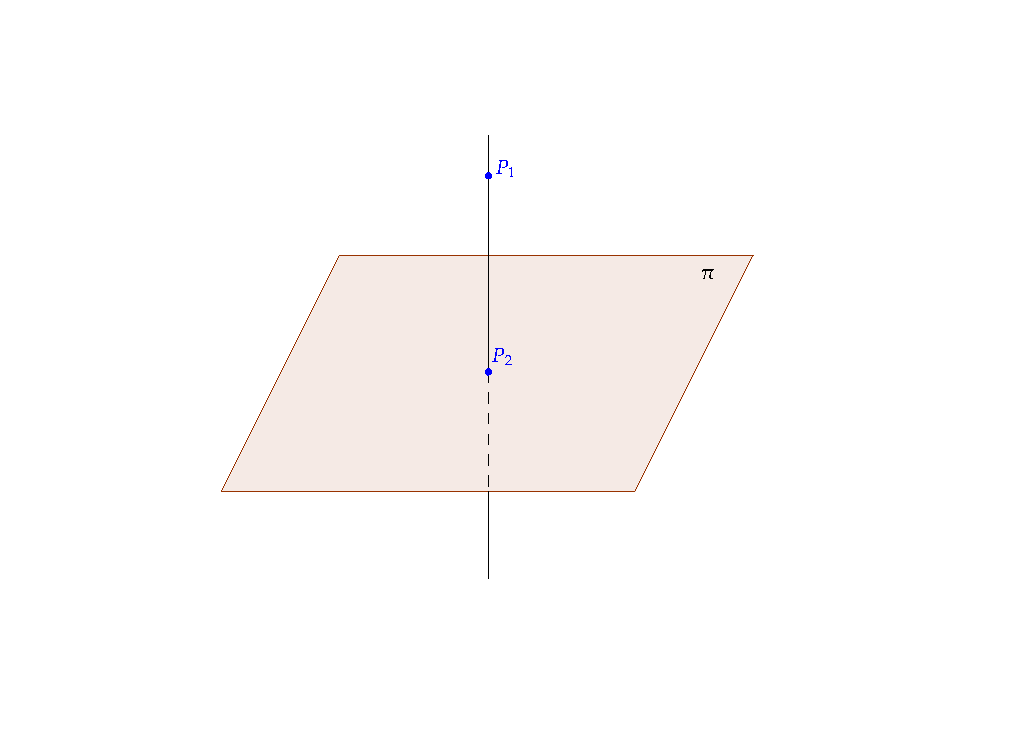
\includegraphics{distancia-ponto-plano.pdf}
    % \definecolor{xdxdff}{rgb}{0.49,0.49,1}
    % \definecolor{zzttqq}{rgb}{0.6,0.2,0}
    % \definecolor{qqqqff}{rgb}{0,0,1}
    % \begin{tikzpicture}[line cap=round,line join=round,>=triangle 45,x=1.0cm,y=1.0cm]
    %     \clip(-4.3,-6.08) rectangle (12.58,6.3);
    %     \fill[color=zzttqq,fill=zzttqq,fill opacity=0.1] (-0.9,-2.02) -- (1.1,1.98) -- (8.1,1.98) -- (6.1,-2.02) -- cycle;
    %     \draw [color=zzttqq] (-0.9,-2.02)-- (1.1,1.98);
    %     \draw [color=zzttqq] (1.1,1.98)-- (8.1,1.98);
    %     \draw [color=zzttqq] (8.1,1.98)-- (6.1,-2.02);
    %     \draw [color=zzttqq] (6.1,-2.02)-- (-0.9,-2.02);

    %     \draw (3.62,0)-- (3.62,4);
    %     \draw [dash pattern=on 5pt off 5pt] (3.62,0)-- (3.62,-2.02);
    %     \draw (3.62,-2.02)-- (3.62,-3.5);
    %     \draw (7.1,1.86) node[anchor=north west] {$\pi$};
    %     \fill [color=qqqqff] (3.62,0) circle (1.5pt);
    %     \draw[color=qqqqff] (3.86,0.26) node {$P_2$};
    %     \fill [color=qqqqff] (3.62,3.32) circle (1.5pt);
    %     \draw[color=qqqqff] (3.92,3.45) node {$P_1$};
    % \end{tikzpicture}
\end{figure}
Seja $r$ a reta que cont\'em o ponto $P_1$ \'e \'e perpendicular ao plano $\pi$. Denote por $P_2(x_2,y_2,z_2)$ a interse\c{c}\~ao de $\pi$ com $r$. O ponto $P_2$ \'e chamado de \textbf{proje\c{c}\~ao ortogonal} de $P_1$ sobre $\pi$. A norma do vetor $\vec{P_1P_2}$ ser\'a a dist\^ancia de $P_1$ a $\pi$, isto \'e,
\[
    d(P_1,\pi) = \norm{\vec{P_1P_2}}.
\]
Seja $\vec{u} = (a,b,c)$ o vetor normal de $\pi$. Como $\vec{u}\varparallel\vec{P_1P_2}$, existe $t \in \real$ tal que
\[
    \vec{P_1P_2} = t\vec{u}.
\]
Logo
\begin{equation}\label{equacaodistanciapontoplano}
    d(P_1,P_2) = \norm{t(a,b,c)} = |t|\sqrt{a^2 + b^2 + c^2}.
\end{equation}
Por outro lado, se $P(x_2, y_2, z_2)$, ent\~ao
\[
    \vec{P_1P_2} = (x_2 - x_1, y_2 - y_1, z_2 - z_1) = t(a,b,c)
\]
e como $P_2 \in \pi$ devemos ter
\[
    a(x_1 + ta) + b(y_1 + tb) + c(z_1 + tc) + d = 0
\]
isto \'e,
\begin{equation}\label{equacaoauxiliardistanciapontoplano}
    t = -\dfrac{ax_1 + by_1 + cz_1 + d_1}{a^2 + b^2 + c^2}.
\end{equation}
Substituindo \eqref{equacaoauxiliardistanciapontoplano} em \eqref{equacaodistanciapontoplano} obtemos
\[
    d(P_1,\pi) = \left|\dfrac{ax_1 + by_1 + cz_1 + d_1}{a^2 + b^2 + c^2}\sqrt{a^2 + b^2 + c^2}\right|
\]
portanto
\[
    d(P_1,\pi) = \dfrac{|ax_1 + by_1 + cz_1 + d_1|}{\sqrt{a^2 + b^2 + c^2}}.
\]

\begin{exemplos}
    \begin{enumerate}
        \item A dist\^ancia entre o plano $\pi: 2x + y - z = 4$ e o ponto $P(1,1,1)$ ser\'a
        \[
            d(P,\pi) = \dfrac{|2 + 1 - 1 - 4|}{\sqrt{4 + 1 + 1}} = \dfrac{2}{\sqrt{6}}.
        \]
        \item Calcule a dist\^ancia entre $\pi_1 : 2x - 3y + z - 2 = 0$ e $\pi_2 : 4x - 6y + 2z - 5 = 0$.
        \begin{solucao}
            Um vetor normal de $\pi_1$ e $\vec{u} = (2,-3,1)$ e de $\pi_2$ \'e $\vec{v} = (4,-6,2)$. Como $\vec{u}\varparallel\vec{v}$, ent\~ao $\pi_1\varparallel\pi_2$ e assim a dist\^ancia entre $\pi_1$ e $\pi_2$ \'e dada pela dist\^ancia de um ponto de $\pi_1$ a $\pi_2$, ou o contr\'ario. Tomando $P_1(1,0,0)\in\pi_1$ temos
            \[
                d(\pi_1,\pi_2) = d(P_1,\pi_2) = \dfrac{|4-5|}{\sqrt{4^2 + (-6)^2 + 2^2}} = \dfrac{1}{\sqrt{56}}.
            \]
        \end{solucao}
    \end{enumerate}
\end{exemplos}

% subsection entre_ponto_e_plano (end)
% section distancias (end)

\subsection{Entre um ponto e uma reta} % (fold)
\label{sub:entre_um_ponto_e_uma_reta}

Seja $P$ um ponto e $r$ uma reta.
\begin{figure}[h]
    \centering
    \caption{Dist\^ancia entre ponto e reta}
    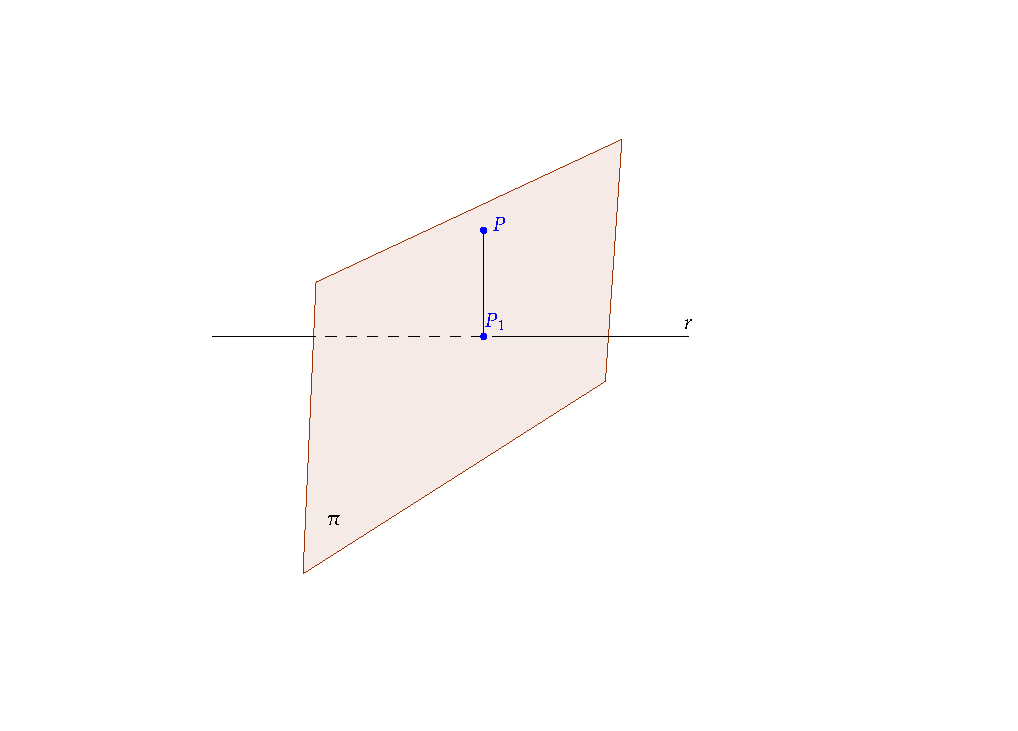
\includegraphics{distancia-ponto-reta.pdf}
    % \definecolor{xdxdff}{rgb}{0.49,0.49,1}
    % \definecolor{zzttqq}{rgb}{0.6,0.2,0}
    % \definecolor{qqqqff}{rgb}{0,0,1}
    % \begin{tikzpicture}[line cap=round,line join=round,>=triangle 45,x=1.0cm,y=1.0cm]
    %     \clip(-4.3,-6.08) rectangle (12.58,6.3);
    %     \fill[color=zzttqq,fill=zzttqq,fill opacity=0.1] (0.48,-3.42) -- (0.7,1.52) -- (5.88,3.94) -- (5.6,-0.16) -- cycle;
    %     \draw [color=zzttqq] (0.48,-3.42)-- (0.7,1.52);
    %     \draw [color=zzttqq] (0.7,1.52)-- (5.88,3.94);
    %     \draw [color=zzttqq] (5.88,3.94)-- (5.6,-0.16);
    %     \draw [color=zzttqq] (5.6,-0.16)-- (0.48,-3.42);
    %     \draw (0.76,-2.3) node[anchor=north west] {$\pi$};
    %     \draw (3.54,2.4)-- (3.54,0.6);
    %     \draw [dash pattern=on 5pt off 5pt] (3.5,0.6)-- (0.65,0.6);
    %     \draw (-1.06,0.6)-- (0.65,0.6);
    %     \draw (3.68,0.6)-- (7,0.6) node[at end,above]{$r$};

    %     \fill [color=qqqqff] (3.54,0.6) circle (1.5pt);
    %     \draw[color=qqqqff] (3.74,0.86) node {$P_1$};
    %     \fill [color=qqqqff] (3.54,2.4) circle (1.5pt);
    %     \draw[color=qqqqff] (3.8,2.5) node {$P$};
    % \end{tikzpicture}
\end{figure}

Para determinar $d(P,r)$ primeiro constru{\'\i}mos um plano $\pi$ passando por $P$ e com vetor normal paralelo ao vetor diretor de $r$. Assim
\[
    d(P,r) = d(P,P_1)
\]
onde $P_1 \in \pi\cap r$.

\begin{exemplo}
    Determinar a dist\^ancia do ponto $P(1,2,-1)$ \`a reta
    \[
        r: \begin{cases}
            x = 1 + 2t\\
            y = 5 - t\\
            z = -2 + 3t.
        \end{cases}
    \]
    \begin{solucao}
        Podemos tomar o vetor $\vec{u} = (2,1,-3)$ como vetor normal ao plano $\pi$ que cont\'em $P$. Da{\'\i}
        \begin{align*}
            \pi &: 2(x - 1) - (y - 2) + 3(z - 1) = 0\\
            \pi &: 2x - y + 3z + 3 = 0.
        \end{align*}
        A interse\c{c}\~ao de $\pi$ com $r$ \'e dada por
        \[
            2(1 + 2t) - (5 - t) + 3(-2 + 3t) = 0,
        \]
        isto \'e, $t = 3/7$ e ent\~ao $P_1(13/7,32/7,-5/7) \in \pi\cap r$. Portanto
        \[
            d(P,r) = d(P,P_1) = \sqrt{\left(1 - \dfrac{13}{7}\right)^2 + \left(2 - \dfrac{32}{7}\right)^2 + \left(-1 + \dfrac{5}{7}\right)^2} = \dfrac{2\sqrt{91}}{7}.
        \]
    \end{solucao}
\end{exemplo}

% subsection entre_um_ponto_e_uma_reta (end)

\subsection{Entre retas} % (fold)
\label{sub:entre_retas}

Sejam $r$ e $s$ retas. Se $r \varparallel s$ ent\~ao a dist\^ancia entre $r$ e $s$ \'e dada pela dist\^ancia entre um ponto de $r$ e a reta $s$, ou o contr\'ario. Suponha ent\~ao que $r$ e $s$ s\~ao reversas. Por um ponto $P$ de $s$ tracemos uma reta $s'$ paralela a $r$.
\begin{figure}[h]
    \centering
    \caption{Dist\^ancia entre retas reversas}
    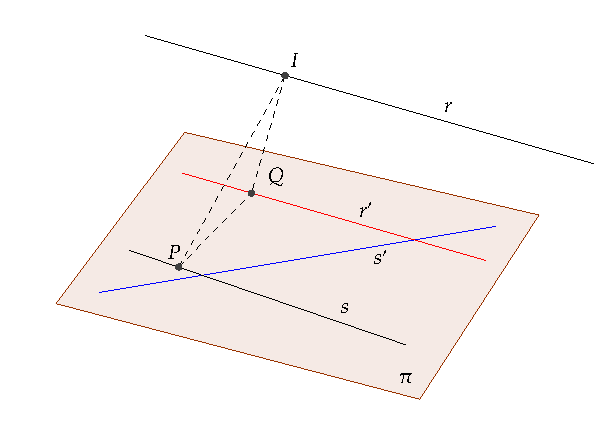
\includegraphics{distancia-retas-reversas.pdf}
    % \definecolor{uququq}{rgb}{0.25,0.25,0.25}
    % \definecolor{xdxdff}{rgb}{0.49,0.49,1}
    % \definecolor{ffqqqq}{rgb}{1,0,0}
    % \definecolor{qqqqff}{rgb}{0,0,1}
    % \definecolor{zzttqq}{rgb}{0.6,0.2,0}
    % \begin{tikzpicture}[line cap=round,line join=round,>=triangle 45,x=1.0cm,y=1.0cm]
    %     \clip(4,-3) rectangle (13.8,4.5);
    %     \fill[color=zzttqq,fill=zzttqq,fill opacity=0.1] (6.6,2.26) -- (4.42,-0.64) -- (10.58,-2.26) -- (12.6,0.86) -- cycle;
    %     \draw [color=zzttqq] (6.6,2.26)-- (4.42,-0.64);
    %     \draw [color=zzttqq] (4.42,-0.64)-- (10.58,-2.26);
    %     \draw [color=zzttqq] (10.58,-2.26)-- (12.6,0.86);
    %     \draw [color=zzttqq] (12.6,0.86)-- (6.6,2.26);
    %     \draw (10.1,-1.7) node[anchor=north west] {$\pi$};
    %     \draw (10.86,2.9) node[anchor=north west] {$r$};
    %     \draw [color=qqqqff] (5.15,-0.45)-- (11.87,0.67);
    %     \draw (5.67,0.26)-- (10.35,-1.34);
    %     \draw [color=ffqqqq] (6.56,1.57)-- (11.7,0.09);
    %     \draw (5.93,3.9)-- (13.52,1.73);
    %     \draw (9.12,-0.5) node[anchor=north west] {$s$};
    %     \draw (9.68,0.4) node[anchor=north west] {$s'$};
    %     \draw (9.42,1.2) node[anchor=north west] {$r'$};
    %     \draw [dash pattern=on 3pt off 3pt] (8.3,3.22)-- (7.73,1.23);
    %     \draw [dash pattern=on 3pt off 3pt] (6.5,-0.02)-- (7.73,1.23);
    %     \draw [dash pattern=on 3pt off 3pt] (6.5,-0.02)-- (8.3,3.22);
    %     \fill [color=uququq] (8.3,3.22) circle (1.5pt);
    %     \draw(8.46,3.48) node {$I$};
    %     \fill [color=uququq] (7.73,1.23) circle (1.5pt);
    %     \draw(7.88,1.5) node[right] {$Q$};
    %     \fill [color=uququq] (6.5,-0.02) circle (1.5pt);
    %     \draw(6.66,0.24) node[left] {$P$};
    % \end{tikzpicture}
\end{figure}

O plano $\pi$ definido por $s$ e $s'$ \'e paralelo a $r$, da{\'\i} a dist\^ancia de $r$ a $\pi$ \'e constante. Esta constante \'e \textbf{a menor dist\^ancia} entre $r$ e $s$. De fato, seja $r'$ uma reta contida em $\pi$ e paralela a $r$. Seja $I$ um ponto de $r$. Por $I$ tracemos um perpendicular a $r$ que a intercepta em um ponto $Q$. Se $P$ \'e um ponto qualquer de $s$ temos
\[
    \overline{IP}^2 = \overline{IQ}^2 + \overline{QP}^2
\]
pois o tri\^angulo $IQP$ \'e ret\^angulo em $Q$. Logo
\[
    \overline{IP}^2 \ge \overline{IQ}^2,
\]
ou seja,
\[
    \overline{IP} \ge \overline{IQ}.
\]
Mas $\overline{IQ}$ \'e a dist\^ancia de $\pi$ a $r$, logo segue da \'ultima desigualdade que a dist\^ancia de $\pi$ a $r$ \'e menor ou igual a dist\^ancia entre um ponto de $r$ e um ponto de $s$. Portanto
\[
    d(r,s) = d(r,\pi).
\]

\begin{exemplo}
    Determine a dist\^ancia entre as retas
    \[
        r: \begin{cases}
            x = 2 + t\\
            y = 1 - 3t\\
            z = 1 + 2t
        \end{cases} \quad s: \begin{cases}
            x = -5 + 4s\\
            y = 6 - 5s\\
            z = 4 + 3s.
        \end{cases}
    \]
    \begin{solucao}
        Os vetores diretores de $r$ e $s$ s\~ao $\vec{u} = (1,-3,2)$ e $\vec{v} = (4,-5,3)$, respectivamente. Logo $r$ e $s$ n\~ao s\~ao paralelas. Agora, o sistema
        \[
            \begin{cases}
                2 + t = -5 + 4s\\
                1 - 3t = 6 - 5s\\
                1 + 2t = 4 + 3s
            \end{cases}
        \]
        e assim $r$ e $s$ s\~ao reversas. Assim pelo ponto $(-5,6,4)$ de $s$ tracemos um reta $s'$ paralela a $r$. Da{\'\i}
        \[
            s' : \begin{cases}
                x = -5 + \alpha\\
                y = 6 - 3\alpha\\
                z = 4 + 2\alpha.
            \end{cases}
        \]
        O vetor $\vec{w} = \vec{u}\times\vec{v}$ \'e perpendicular ao plano definido por $s$ e $s'$. Como $\vec{w} = (1,5,7)$ ent\~ao o plano $\pi$ contendo $s$ e $s'$ \'e dado por
        \[
            \pi : x + 5y + 7z - 53 = 0.
        \]
        Finalmente, seja $P(2,1,1) \in r$. Ent\~ao
        \[
            d(r,s) = d(P,\pi) = \dfrac{|2 + 5 + 7 - 53|}{\sqrt{1 + 5^2 + 7^2}} = \dfrac{39}{\sqrt{75}}.
        \]


    \end{solucao}
\end{exemplo}
% subsection entre_retas (end)

% chapter reta_e_plano_no_espaco (end)
